\chapter{Data Model}\label{ch:datamodel}

\figref{fig:datamodel} shows the analysis classes of the data model used by the
application.

\begin{figure}[htb]
	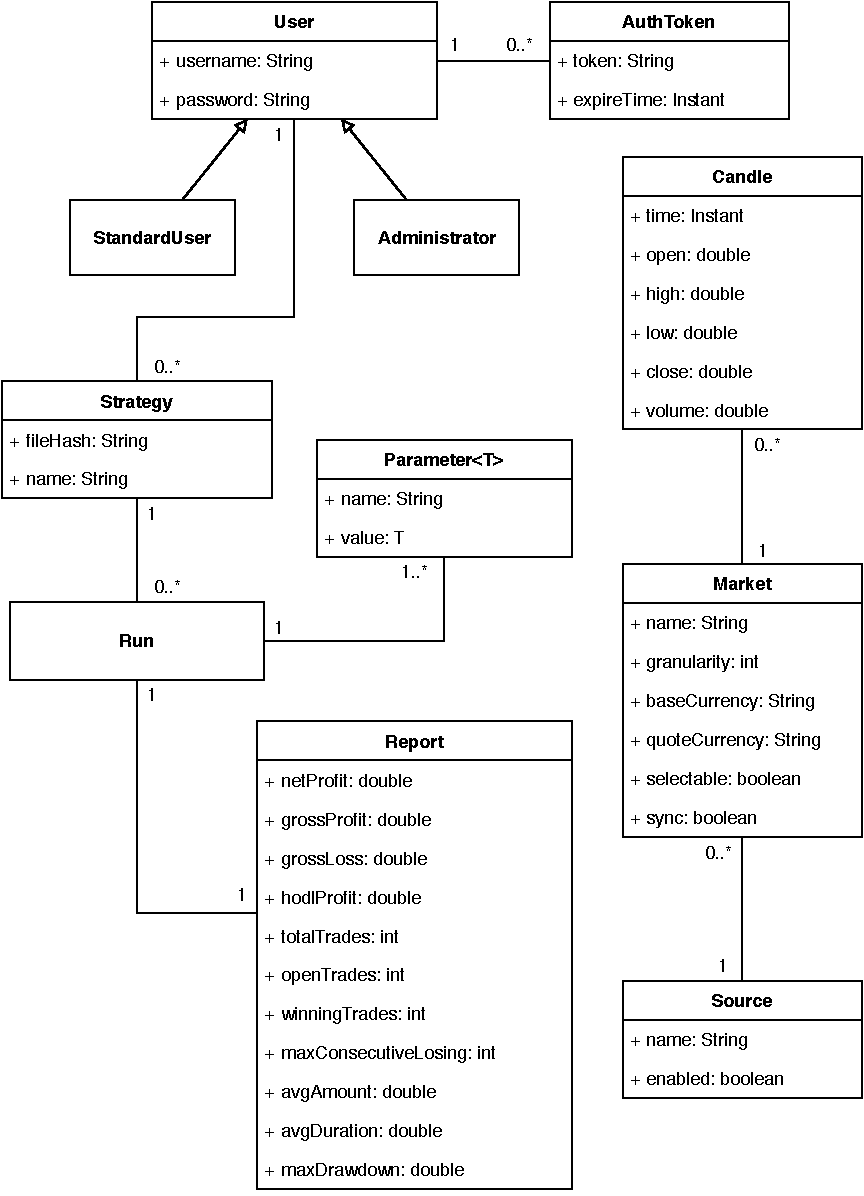
\includegraphics[width=\textwidth,height=\dimexpr\textheight-14\baselineskip,keepaspectratio]{datamodel}
	\caption{Data model UML diagram (analysis classes).}\label{fig:datamodel}
\end{figure}

\section{Collections}\label{sec:collections}

In this section we will define the database structure. The following collections
are defined:
\begin{enumerate*}[label=]
	\item \code{Users};
	\item \code{MarketData};
	\item \code{Sources};
	\item \code{Strategies}.
\end{enumerate*}

\subsection{Users}

\lstinputlisting[language=json, label={lst:userscollection},
caption={\code{User} document example.}]{users.json}

Each document represents a user.

Fields' description:
\begin{description}
	\item[\_id] \textit{(string)} Username;
	\item[password] \textit{(string)} Password hash;
	\item[is\_admin] \textit{(boolean, optional)} Specifies whether the user
		is the administrator or not; if not present, is considered
		\code{false};
	\item[auth\_token] \textit{(array, optional)} Array of embedded
		documents that represent the tokens used to authenticate the
		user with the server. This is an array since multiple clients
		can connect as the same user creating a session (a token) for
		each client (this allows for a session management feature to be
		implemented in future). The structure of these documents is the
		following:
		\begin{description}
			\item[token] \textit{(string)} Token hash (generated
				randomly);
			\item[expire\_time] \textit{(timestamp)} Token expire
				time.
		\end{description}
\end{description}

\subsection{MarketData}

\lstinputlisting[language=json, label={lst:marketdatacollection},
caption={\code{MarketData} document example.}]{marketdata.json}

Each document represents a month of a market.

Fields' description:
\begin{description}
	\item[\_id] \textit{(ObjectId)} An unique id automatically generated by
		the database;
	\item[market] \textit{(string)} Identifies the market. Format:
		\code{sourcename:market\-name};
	\item[month] \textit{(string)} Year and month of the trading days
		available in this document. Format: \code{YYYY-MM};
	\item[data] \textit{(array)} Array of embedded documents where each
		document represent a trading day. This array is pre-filled at
		the start of every month (it can not be empty). The structure of
		these documents is the following:
		\begin{description}
			\item[t] \textit{(timestamp)} The closing time of the
				day;
			\item[o] \textit{(numeric)} The opening price of the
				day;
			\item[h] \textit{(numeric)} The highest price of the
				day;
			\item[l] \textit{(numeric)} The lowest price of the day;
			\item[c] \textit{(numeric)} The closing price of the
				day;
			\item[v] \textit{(numeric)} The volume, \idest*{the
				amount traded during the day}.
		\end{description}
\end{description}

\subsection{Sources}

\lstinputlisting[language=json, label={lst:sourcescollection},
caption={\code{Sources} document example.}]{sources.json}

Each document represents a data source.

Fields' description:
\begin{description}
	\item[\_id] \textit{(string)} Source name;
	\item[enabled] \textit{(boolean, optional)} Specifies if users are
		allowed or not to test strategies on the markets of this data
		source. If not present, is considered \code{true};
	\item[streaming] \textit{(boolean, optional)} Specifies if the streaming
		from this data source is enabled or not. If not present, is
		considered \code{false}. If \code{enabled} is \code{false}, this
		is considered \code{false};
	\item[api\_key] \textit{(string, optional)} The API key used by the
		scraper to access the API endpoint. If not present, no API key
		is used;
	\item[markets] \textit{(array, optional)} array of embedded documents
		that lists the market available for this source. The structure
		of these documents is the following:
		\begin{description}
			\item[\_id] \textit{(string)} Name of the market;
			\item[granularity] \textit{(integer)} Minimum size,
				in minutes, of the trading day.
			\item[enabled] \textit{(boolean, optional)} Specifies if
				users are allowed or not to test strategies on
				this market. If not present, is considered
				\code{true}. If source's \code{enabled} is
				\code{false}, this is considered \code{false}.
		\end{description}
\end{description}

\subsection{Strategies}

\lstinputlisting[language=json, label={lst:strategiescollection},
caption={\code{Strategies} document example.}]{strategies.json}

Each document represents a strategy.

Fields' description:
\begin{description}
	\item[\_id] \textit{(string)} Hash of the file that defines the
		strategy;
	\item[runs] \textit{(array, optional)} Array of embedded documents that
		list all the tests made by the users with this strategy. The
		structure of these documents is the following:
		\begin{description}
			\item[config] \textit{(document)} Strategy's
				configuration used:
				\begin{description}
					\item[time]
						\textit{(timestamp)} Time of the
						last data on which the strategy
						has been executed;
					\item[market] \textit{(string)} Name of
						the market on which the strategy
						has been executed. Format:
						\enquote{sourcename:marketname};
					\item[granularity] \textit{(integer)}
						Trading day aggregation factor
						(this value is multiplied to the
						minimum granularity in order to
						obtain a higher level of
						aggregation);
					\item[\ldots] Other fields may be
						present (defined by the
						strategy).
				\end{description}
			\item[report] \textit{(document)} Report generated by
				the execution of the strategy:
				\begin{description}
					\item[net\_profit] \textit{(numeric)}
						The profit of the strategy,
						computed as the total profit
						minus the total loss of the
						trades (percentage of the
						initial amount);
					\item[gross\_profit] \textit{(numeric)}
						The total profit of the
						strategy, not counting the
						losing trades (percentage of the
						initial amount);
					\item[max\_drawback] \textit{(numeric)}
						The maximum drawback as defined
						in \chref{ch:specs}. This is
						expressed as a percentage of the
						initial amount;
					\item[hodl\_profit] \textit{(numeric)}
						The profit (\(\ge 1\)) or
						loss (\(< 1\)) of the Buy and
						Hold strategy (percentage of the
						initial amount).
					\item[trades] \textit{(array, optional)}
						Array of embedded documents that
						describes the transactions made
						by the strategy. The structure
						of these documents is the
						following:
						\begin{description}
							\item[entry\_time]
								\textit{(timestamp)}
								The time at
								which the trade
								is initiated;
							\item[exit\_time]
								\textit{(timestamp,
								optional)}
								The time at
								which the trade
								is concluded
								(not present if
								still open);
							\item[amount]
								\textit{(numeric)}
								The amount of
								asset traded.
								This is a value
								between 0 and 1
								(percentage of
								the initial
								amount);
							\item[profit]
								\textit{(numeric,
								optional)} The
								profit (\(\ge
								1\)) or loss
								(\(< 1\)) of the
								trade, expressed
								as a percentage
								of the traded
								amount (not
								present if the
								trade is still
								open).
						\end{description}
				\end{description}
		\end{description}
\end{description}

\section{Indexes}\label{sec:indexes}

To ensure better performance of the application, some indexes are defined for
each collection.

Note that, during the development of the application, some of the following
indexes may be changed, removed, or other indexes may be added. Those decisions
will be guided by performance evaluations of the application on common
workloads.

\subsection{AuthTokens}

Auth tokens are always retrieved by the token hash, which is saved in the
\code{\_id} field that is already an unique index.

Additionally, the following \standout{TTL index} is defined:

\begin{lstlisting}[language=json]
{"expireTime": 1}, {expireAfterSeconds: 0}
\end{lstlisting}

This will instruct \mongodb{} to automatically remove tokens when they expire.

Note that in order to define a TTL index we can not save the auth tokens as
embedded documents inside the \code{Users} collection since indexes in
\mongodb{} are always \emph{collection-level} (so, setting a TTL index in an
embedded document, will result in the deletion of the entire root document when
the TTL expires).

\subsection{Sources}

We need to get a source, with all the markets, or a single market inside a
source. The following \standout{compound unique} index can support both queries:

\begin{lstlisting}[language=json]
{"_id": 1, "markets.id": 1}, {unique: true}
\end{lstlisting}

We may exploit the \mongodb's index intersection feature to support the query
that gets a single market, but since there is no need to get all the markets
with a specific \code{id} from all sources (we always get a specific market in a
specific source), we prefer to define a compound index in order to save
\mongodb{} the need to access two indexes to perform the query. Moreover, this
index enforces the uniqueness of the combination of the two fields.

\subsection{MarketData}

We need to get market data by \code{market} during the execution of a strategy.
We define an \standout{hashed index} on the \code{market} field:

\begin{lstlisting}[language=json]
{"market": "hashed"}
\end{lstlisting}

This is an hashed index since it will also be used as a shard key to shard the
collection over multiple servers, as defined in \secref{sec:distributed}.

Moreover, we need to sort documents based on the \code{start} field:

\begin{lstlisting}[language=json]
{"start": 1}
\end{lstlisting}

The \code{start} field is a redundancy since it has the same value of the
\code{t} field of the first candle in the document (\code{candles.0.t}). The
redundancy is added just to create this index to improve the sorting operation
(we could have set an index on \code{candles.t}, but this would have caused the
side effect of creating an index entry for each candle which is useless).

\subsection{Strategies}

Strategies are retrieved by file hash (the \code{\_id} field, already indexed)
or by name. Thus, we define the following \standout{unique index}:

\begin{lstlisting}[language=json]
{"name": 1}, {unique: true}
\end{lstlisting}

Since we also need to retrieve a specific run of a strategy, we also define the
following:

\begin{lstlisting}[language=json]
{"runs.id": 1}, {unique: true, sparse: true}
\end{lstlisting}

The uniqueness ensures that we can get a run using just its \code{id} and
without specifying which strategy it belongs to.

The index is \emph{sparse} since we do not want to index strategies that does
not have any run in the \code{runs} array.

To allow the application to rapidly sort strategy's reports by the net profit
(commonly used to represent the overall performance of a strategy), we define
the following index:

\begin{lstlisting}[language=json]
{"runs.report.netProfit": 1}
\end{lstlisting}

\section{Aggregation Pipelines}\label{sec:aggregations}

The following \standout{Aggregation Pipelines} has been defined:

\begin{itemize}
	\item To obtain a larger granularity on the data present in a given
		market, when we apply a strategy, we can aggregate the
		documents contained in the \code{data} array in the
		\code{MarketData} collection:
		\begin{enumerate}
			\item \code{\$match} stage to get the document
				containing the data for the specific market and
				the current month. This stage includes the
				entire shard key, so it is directed only to the
				specific server where the shard containing the
				document is saved;
			\item \code{\$project} stage to exclude the \code{\_id}
				field, no longer needed;
			\item \code{\$unwind} stage to extract the documents in
				the \code{data} field;
			\item \code{\$bucket} stage to aggregate multiple
				documents based on ranges of the \code{t} field.
		\end{enumerate}
	\item The server needs to know what is the first month for which data is
		available for a specific market, in order to run a query on that
		market. The following pipeline on the \code{MarketData}
		collection is defined:
		\begin{enumerate}
			\item \code{\$match} stage selects all documents for a
				specific market;
			\item \code{\$project} stage to extract only the
				\code{\_id} field, since the \code{data} field
				is not needed;
			\item \code{\$sort} stage to sort all documents by
				\code{\_id};
			\item \code{\$group} stage to get the value of the
				\code{\_id} field of the first document.
		\end{enumerate}
	\item At the start, the scraper needs to know the
		first and last month for which data is available for each
		market, in order to determine the range of data already
		available and restart downloading the data that is outside of
		this range. The following pipeline on the \code{MarketData}
		collection, similar to the previous one, is defined:
		\begin{enumerate}
			\item \code{\$project} stage to extract only the
				\code{\_id} field, since the \code{data} field
				is not needed. Moreover, in this stage, the
				\code{\_id} field is split into two fields: the
				first (\code{market}) contains the source name
				concatenated with the market name; the second
				(\code{month}) contains the string representing
				the year and the month;
			\item \code{\$sort} stage to sort all documents by
				\code{month};
			\item \code{\$group} stage to aggregate all documents
				by the same \code{market} and get the first and
				last document for each market;
			\item \code{\$poject} stage to output only the needed
				values (the first and last month).
		\end{enumerate}
	\item Further aggregations may be defined in future. In particular,
		other aggregations probably may be needed during the development
		of the functions used by strategies to get statistics over the
		market data. Moreover, during the development of the
		application, the need for other aggregations may arise.
\end{itemize}

Note that, during the development of the application, the above pipelines may be
implemented in some other way \exgratia{different stages or in different order}
in order to improve the performance of the queries.

